\chapter{CALIDAD Y SEGURIDAD} 
\section{CALIDAD DE SOFTWARE}
\subsection{Usabilidad}

La usabilidad se evaluará a través de la escala de Likert, la cual permitirá medir la cantidad de clics necesarios para realizar distintas tareas en el software. De esta manera, se podrá valorar el nivel de satisfacción de los usuarios respecto al número de clics requeridos para completar dichas tareas. Además, esta escala proporcionará una visión clara sobre la eficiencia del diseño del software, ayudando a identificar áreas que podrían necesitar ajustes para mejorar la experiencia del usuario. La escala se define de la siguiente manera:

\begin{itemize}[label=$-$, left=0cm, labelsep = 0.9cm, topsep = 0pt, parsep = 0pt]
	\item \textbf{Muy insatisfecho:} Cinco o más clics, ya que las tareas requieren demasiados clics y son consideradas tediosas.		
	\item \textbf{Insatisfecho:} Cuatro clics, lo que indica que la tarea requiere más clics de los deseados y resulta algo incómoda.
	\item \textbf{Neutral:} Tres clics, una cantidad aceptable, aunque con margen de mejora.
	\item \textbf{Satisfecho:} Dos clics, considerado un número razonable que permite realizar la tarea de manera eficiente.
	\item \textbf{Muy satisfecho:} Un clic, ideal por ser altamente eficiente y requerir el mínimo esfuerzo.
\end{itemize}

\begin{longtable}{>{\centering\arraybackslash}m{5cm} >{\centering\arraybackslash}m{3cm} >{\centering\arraybackslash}m{3cm}}
	\caption[Número de Clics - Escala Likert]{\newline Número de Clics - Escala Likert} \label{tab:tabla_clics}\\
	\toprule
	\textbf{Tarea} & \textbf{Clics} & \textbf{Puntos}\\
	\midrule
	\endfirsthead
	
	\toprule
	\textbf{Tarea} & \textbf{Clics} & \textbf{Puntos}\\
	\midrule
	\endhead
	
	%\midrule
	%\multicolumn{3}{r}{\textit{Continúa en la siguiente página}} \\
	%\midrule
	%\endfoot
	
	\bottomrule
	\endlastfoot
	
	% Aquí se colocan las filas de la tabla, por ejemplo:
	Ingresar usuario      & 2 & 2 \\
	Registrar usuario     & 3 & 3 \\
	Registrar cliente     & 4 & 4 \\
	Venta de pasaje       & 3 & 3 \\
	Cancelar pasaje       & 2 & 2 \\
	Registrar encomienda  & 4 & 4 \\
	Generar reporte		  & 2 & 2 \\
	Cerrar sesión		  & 1 & 1 \\ \hline
	Total				  & 21 &  \\ \hline
	Promedio 			  &   & 2.62 \\
	
\end{longtable}
\vspace{-12pt}  % O el valor que necesites para ajustar
% Nota personalizada fuera de `\caption*{}`
\textbf{Nota}: Resultados obtenidos a partir de la escala Likert sobre la cantidad de clics necesarios para ejecutar tareas comunes.

Se tiene un total de 21 clics para las tareas realizadas, con esto número obtenemos el promedio de clics de 2.62 y con este resultado concluimos que la usabilidad del sistema es "Satisfactorio".

\subsection{Portabilidad}

El proyecto es compatible con navegadores modernos asegurando una experiencia uniforme mediante el uso de estándares web, esto permite que el sistema funcione de manera consistente en distintos entornos, facilitando su acceso desde cualquier dispositivo. Se han implementado medidas para optimizar el rendimiento y minimizar inconsistencias entre navegadores, garantizando una experiencia fluida y eficiente para todos los usuarios, como podemos ver en las figuras \ref{fig:figura_brave}, \ref{fig:figura_edge} y \ref{fig:figura_celular}.

\vspace{3cm} % Agregar 1 cm de espacio entre el párrafo y la figura

\begin{figure}[!h] % 'H' del paquete 'float' para mantener posición	
	\caption[Navegador Brave]
	{\newline Navegador Brave.} % Leyenda en la parte superior
	\centering
	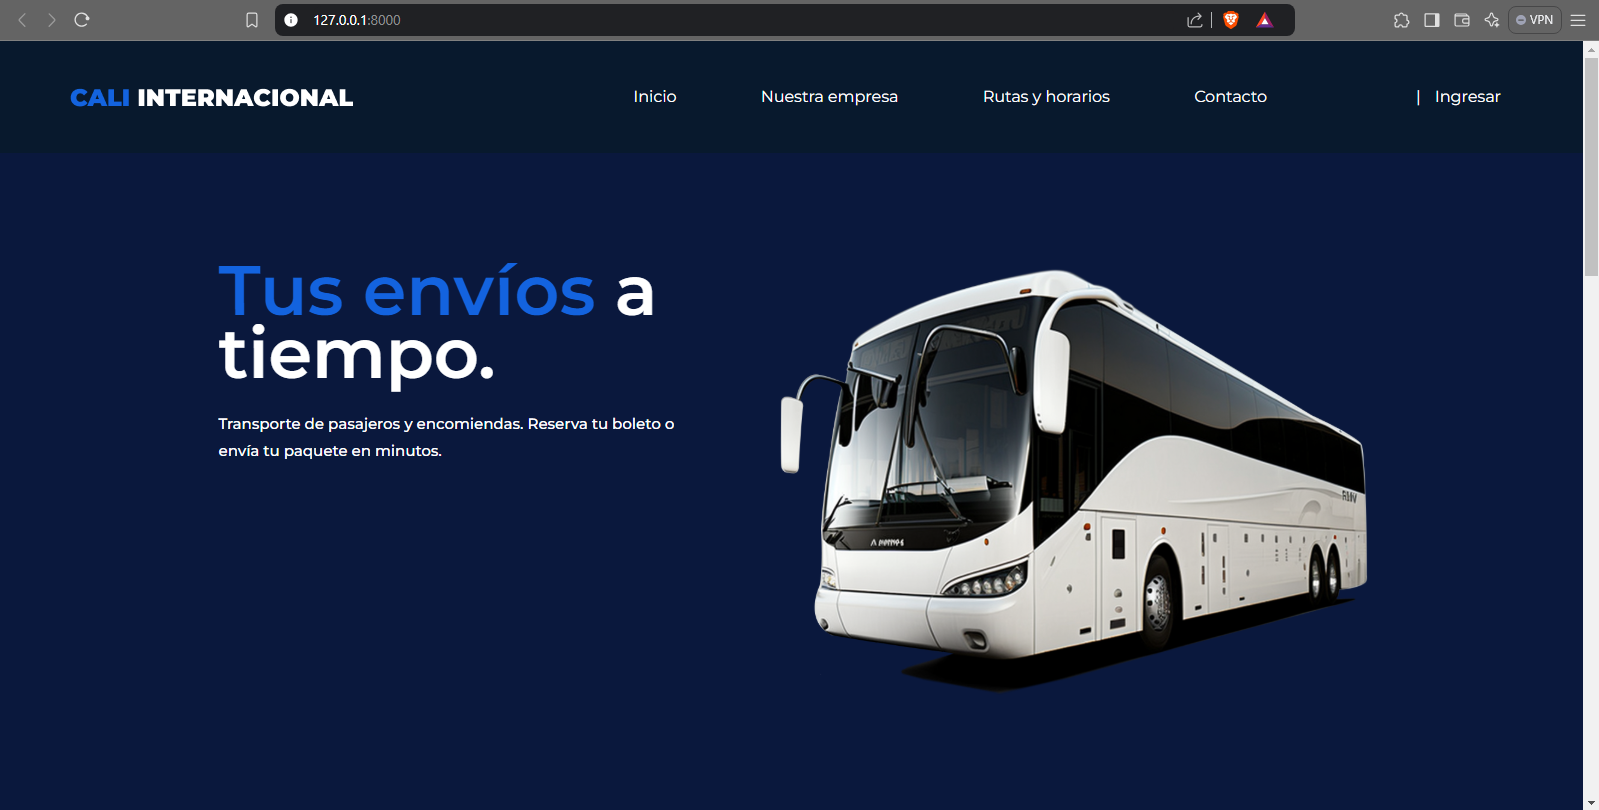
\includegraphics[width=0.85\textwidth]{imagenes/cap_3/brave.png} % Inserta una imagen
	\begin{flushleft}
		\hspace{1.20cm} \textit{Nota.} Visualización correcta del sistema en el navegador Brave. % Nota al pie para esta figura
	\end{flushleft}
	\vspace{-16pt}
	\label{fig:figura_brave} % Etiqueta para referencia cruzada
\end{figure}

%\vspace{1cm} % Agregar 1 cm de espacio entre el párrafo y la figura

\begin{figure}[!h] % 'H' del paquete 'float' para mantener posición	
	\caption[Navegador Microsoft Edge]
	{\newline Navegador Microsoft Edge.} % Leyenda en la parte superior
	\centering
	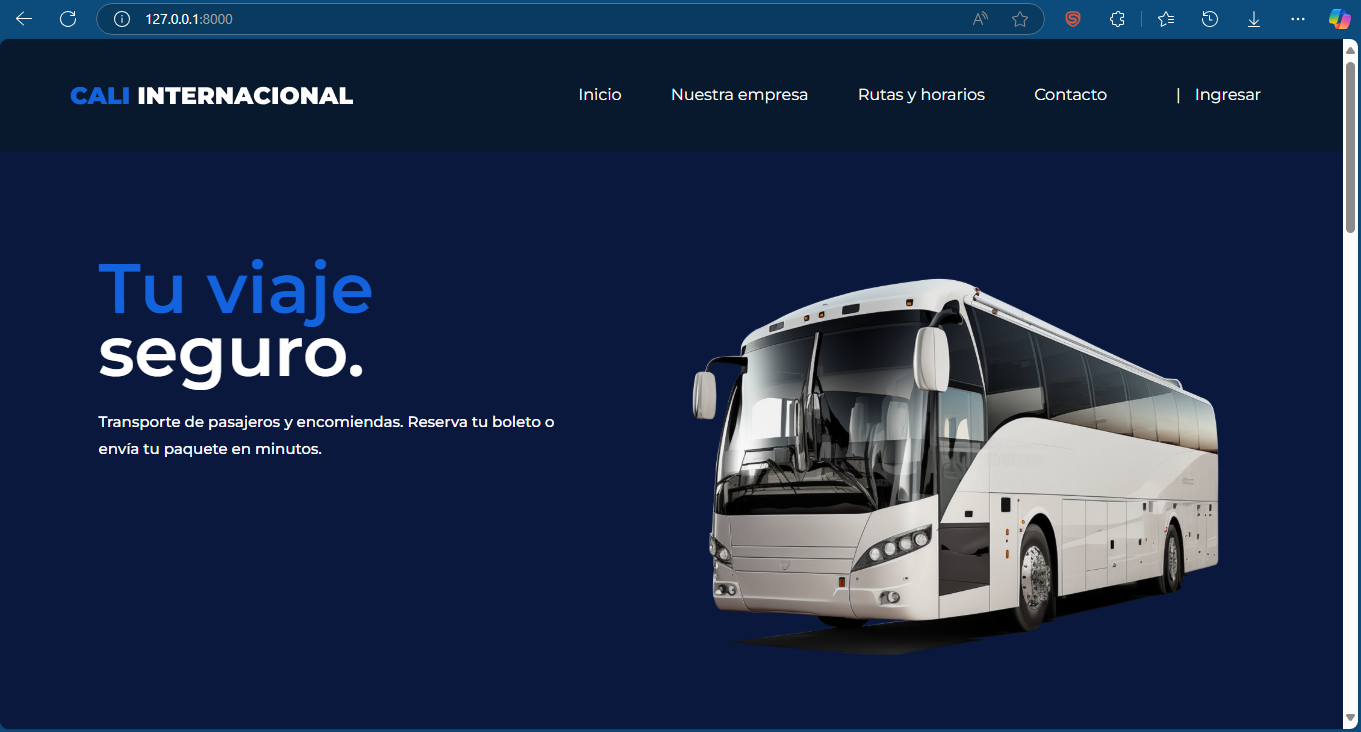
\includegraphics[width=0.85\textwidth]{imagenes/cap_3/edge.png} % Inserta una imagen
	
	\begin{flushleft}
		\hspace{1.20cm} \textit{Nota.} Compatibilidad del sistema con Microsoft Edge. % Nota al pie para esta figura
	\end{flushleft}
	\vspace{16pt}
	\label{fig:figura_edge} % Etiqueta para referencia cruzada
\end{figure}

%\vspace{6cm} % Agregar 1 cm de espacio entre el párrafo y la figura

\begin{figure}[!h] % 'H' del paquete 'float' para mantener posición	
	\caption[Navegador Chrome - Móvil]
	{\newline Navegador Chrome - Móvil.} % Leyenda en la parte superior
	\centering
	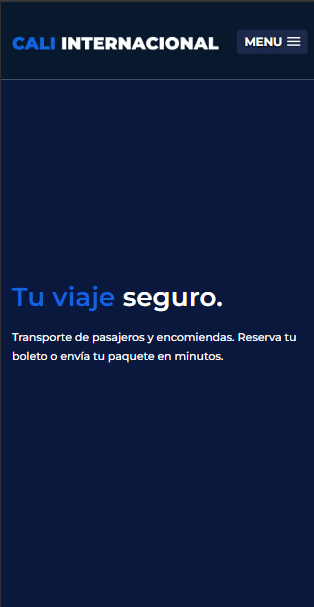
\includegraphics[width=0.4\textwidth]{imagenes/cap_3/celular.png} % Inserta una imagen
	
	\begin{flushleft}
		\hspace{1.20cm} \textit{Nota.} Prueba de portabilidad en el navegador Chrome en un móvil. % Nota al pie para esta figura
	\end{flushleft}
	\vspace{-16pt}
	\label{fig:figura_celular} % Etiqueta para referencia cruzada
\end{figure}

\vspace{0.3cm} % Agregar 1 cm de espacio entre el párrafo y la figura

\subsection{Mantenibilidad}

	Esta característica se refiere a la facilidad con la que se pueden realizar modificaciones en la interfaz del sistema, ya sea para aplicar correcciones, introducir mejoras o adaptarse a cambios en el entorno o en los requerimientos funcionales. Para evaluar la calidad del mantenimiento del sistema, se utilizará el Índice de Madurez del Software (IMS), el cual refleja el nivel de estabilidad de la aplicación. Este índice se calcula restando la cantidad de módulos añadidos, modificados y eliminados del total de módulos del sistema, y dividiendo el resultado entre ese mismo total.
	
	\[
		\text{IMS} = \frac{M_T - (F_a + F_c + F_d)}{M_T}
	\]
	
	Donde:
	
	\begin{flushleft}
		\begin{itemize}
			\item $M_T$ = 9 módulos totales
			\item $F_a$ = 0 módulos que se modificaron
			\item $F_c$ = 1 módulo agregado
			\item $F_d$ = 0 módulos eliminados
		\end{itemize}
	\end{flushleft}
	
	Entonces:
	
	\[
		\text{IMS} = \frac{15 - (0 + 1 + 0)}{15} = 0.88
	\]
	
	Con ese resultado se concluye que el sistema, tiene un índice de madurez de software del 88 por ciento%.
	
\section{SEGURIDAD}

	La seguridad informática constituye un componente esencial en el desarrollo de cualquier sistema de información, especialmente cuando se gestionan datos personales, operaciones comerciales y registros de transacciones. En ese sentido, es fundamental establecer mecanismos que garanticen que la información no sea comprometida por accesos no autorizados, modificaciones indebidas o pérdidas accidentales.
	
	El presente sistema fue diseñado aplicando buenas prácticas de seguridad tanto en el desarrollo del software como en su configuración, con el propósito de proteger la confidencialidad, integridad y disponibilidad de los datos. A continuación, se describen los principales mecanismos de seguridad implementados.

\subsection{Autenticación y control de acceso}

	El sistema implementa un mecanismo de autenticación de usuarios basado en el módulo django.contrib.auth, que permite el uso de nombres de usuario y contraseñas seguras para iniciar sesión. Asimismo, se aplica un esquema de control de acceso por roles, permitiendo que diferentes tipos de usuarios (administradores, empleados) tengan acceso únicamente a las funcionalidades que les corresponden.
	
	Se utiliza el siguiente código para proteger las vistas mediante autenticación:
	
	\textbf{Programa 3.17}
	
	\textit{Protección de vistas mediante autenticación y permisos.} % Título y subtítulo alineados
	\vspace{0.3cm} % Espaciado opcional entre el título y el código
	\begin{lstlisting}[lineskip=-1pt]
		from django.contrib.auth.mixins import LoginRequiredMixin, PermissionRequiredMixin
		from django.views.generic import ListView
		from .models import Parcel
		
		class ParcelListView(LoginRequiredMixin, PermissionRequiredMixin, ListView):
			model = Parcel
			permission_required = 'app.view_parcel'
			template_name = 'parcel/list.html'
	\end{lstlisting}
	
	\textbf{Nota:} Parte del código que muestra como restringir el acceso a una vista de lista de encomiendas.

	Con este enfoque, los usuarios no autenticados o sin permisos adecuados son redirigidos o bloqueados automáticamente.
	
\subsection{Almacenamiento seguro de contraseñas}
	
	Las contraseñas de los usuarios no se almacenan en texto plano, lo cual representa una medida de seguridad fundamental para evitar el compromiso de credenciales en caso de una filtración de datos. El framework Django implementa, por defecto, el algoritmo PBKDF2 con el hash SHA256 para proteger las contraseñas almacenadas en la base de datos. Este algoritmo pertenece a la familia de funciones derivadas de clave y está diseñado para ser computacionalmente intensivo, lo cual dificulta la posibilidad de realizar ataques de fuerza bruta o ataques de diccionario a gran escala.
	
	Además de aplicar un hash robusto, el sistema cuenta con una configuración de validadores de contraseñas definida en el archivo settings.py, la cual tiene como propósito fortalecer aún más la seguridad desde el momento en que el usuario crea o actualiza su contraseña. Esta configuración permite evitar contraseñas débiles o predecibles, tales como combinaciones numéricas simples, nombres comunes o contraseñas que guarden similitud con el nombre de usuario u otros atributos personales. De esta forma, se fomenta el uso de credenciales más complejas y difíciles de vulnerar, alineándose con las buenas prácticas de seguridad recomendadas por la comunidad de desarrollo de software.
	
	\textbf{Programa 3.18}
	
	\textit{Validadores de contraseñas en la configuración del sistema.} % Título y subtítulo alineados
	\vspace{0.3cm} % Espaciado opcional entre el título y el código
	\begin{lstlisting}[lineskip=-1pt]
		AUTH_PASSWORD_VALIDATORS = [
		{
			'NAME': 'django.contrib.auth.password_validation.UserAttributeSimilarityValidator',
		},
		{
			'NAME': 'django.contrib.auth.password_validation.MinimumLengthValidator',
			'OPTIONS': { 'min_length': 8 }
		},
		{
			'NAME': 'django.contrib.auth.password_validation.CommonPasswordValidator',
		},
		{
			'NAME': 'django.contrib.auth.password_validation.NumericPasswordValidator',
		},
		]
		
	\end{lstlisting}
	
	\textbf{Nota:} Este fragmento representa la configuración para garantizar contraseñas seguras.
	
\subsection{Prevención de ataques comunes}

	Django incluye múltiples mecanismos de protección contra amenazas web conocidas:
	
	CSRF (Cross-Site Request Forgery): Todos los formularios incluyen automáticamente un token CSRF. Esto evita que se realicen acciones no autorizadas desde otros sitios web.
	
	XSS (Cross-Site Scripting): El motor de plantillas de Django escapa automáticamente el contenido inyectado, evitando que scripts maliciosos se ejecuten en el navegador.
	
	Inyección SQL: Las consultas a la base de datos se realizan mediante el ORM de Django, el cual utiliza parámetros protegidos contra inyección.
	
	Uso de token CSRF en formularios HTML:

	\textbf{Programa 3.20}
	
	\textit{Uso del token CSRF en formularios HTML en Django.} % Título y subtítulo alineados
	\vspace{0.3cm} % Espaciado opcional entre el título y el código
	\begin{lstlisting}[lineskip=-1pt]
		<form method="post">
			
			<div class="form-group">
				<label for="origen">Ciudad de Origen:</label>
				<input type="text" name="origen" class="form-control" required>
			</div>
			<div class="form-group">
				<label for="destino">Ciudad de Destino:</label>
				<input type="text" name="destino" class="form-control" required>
			</div>
			<button type="submit" class="btn btn-primary">Crear Ruta</button>
		</form>		
	\end{lstlisting}
	
	\textbf{Nota:} Aqui se ilustra cono insertar el token CSRF en formularios.
	
\subsection{Seguridad en la transmisión de datos}
	
	Para proteger la información transmitida entre el cliente y el servidor, el sistema puede configurarse para funcionar sobre HTTPS, utilizando un certificado SSL. Esto asegura que los datos sensibles, como credenciales o transacciones, estén cifrados. El uso de HTTPS no solo protege contra ataques de tipo man-in-the-middle, sino que también garantiza la autenticidad del servidor al que se conecta el usuario. Además, el sistema puede ser configurado para redirigir automáticamente todas las solicitudes HTTP a HTTPS, reforzando así una política de comunicación segura de extremo a extremo.
	
	En el entorno de producción, se recomienda activar las siguientes configuraciones en settings.py:

	\textbf{Programa 3.21}
	
	\textit{Configuración de seguridad para HTTPS.} % Título y subtítulo alineados
	\vspace{0.3cm} % Espaciado opcional entre el título y el código
	\begin{lstlisting}[lineskip=-1pt]
		SECURE_SSL_REDIRECT = True
		SESSION_COOKIE_SECURE = True
		CSRF_COOKIE_SECURE = True
		SECURE_HSTS_SECONDS = 31536000
		SECURE_HSTS_INCLUDE_SUBDOMAINS = True
		SECURE_HSTS_PRELOAD = True
	\end{lstlisting}
	
	\textbf{Nota:} Este bloque corresponde a las configuraciones para asegurar la transmisión de datos cifrada.

	Estas medidas fortalecen la seguridad contra ataques de tipo man-in-the-middle y aseguran el uso exclusivo de conexiones cifradas.

\subsection{Gestión de sesiones}

	Para evitar el uso indebido de sesiones abiertas o caducadas, se establecen configuraciones como:
	
	\textbf{Programa 3.22}
	
	\textit{Configuración del tiempo de expiración de sesiones.} % Título y subtítulo alineados
	\vspace{0.3cm} % Espaciado opcional entre el título y el código
	\begin{lstlisting}[lineskip=-1pt]
		# Configuración de sesiones
		SESSION_COOKIE_AGE = 1800  # 30 minutos
		SESSION_EXPIRE_AT_BROWSER_CLOSE = True
		SESSION_COOKIE_HTTPONLY = True
		SESSION_COOKIE_SAMESITE = 'Strict'
		SESSION_SAVE_EVERY_REQUEST = True
	\end{lstlisting}
	
	\textbf{Nota:} Este código define el tiempo de vida de las sesiones en el sistema.
	
	Esto garantiza que las sesiones se cierren automáticamente después de un período de inactividad o al cerrar el navegador.
	
\subsection{Auditoría y registro de actividades}

	El sistema puede registrar eventos relevantes como inicios de sesión, creación de rutas, ventas de pasajes y gestión de encomiendas, ya sea utilizando los logs estándar de Django o con bibliotecas como django-simple-history o django-auditlog.
	
	Esto permite rastrear comportamientos sospechosos, recuperar historial y facilitar auditorías internas.
	
	 \begin{figure}[!h] % 'H' del paquete 'float' para mantener posición	
		\caption[Lista de accesos]
		{\newline Lista de accesos.} % Leyenda en la parte superior
		\centering
		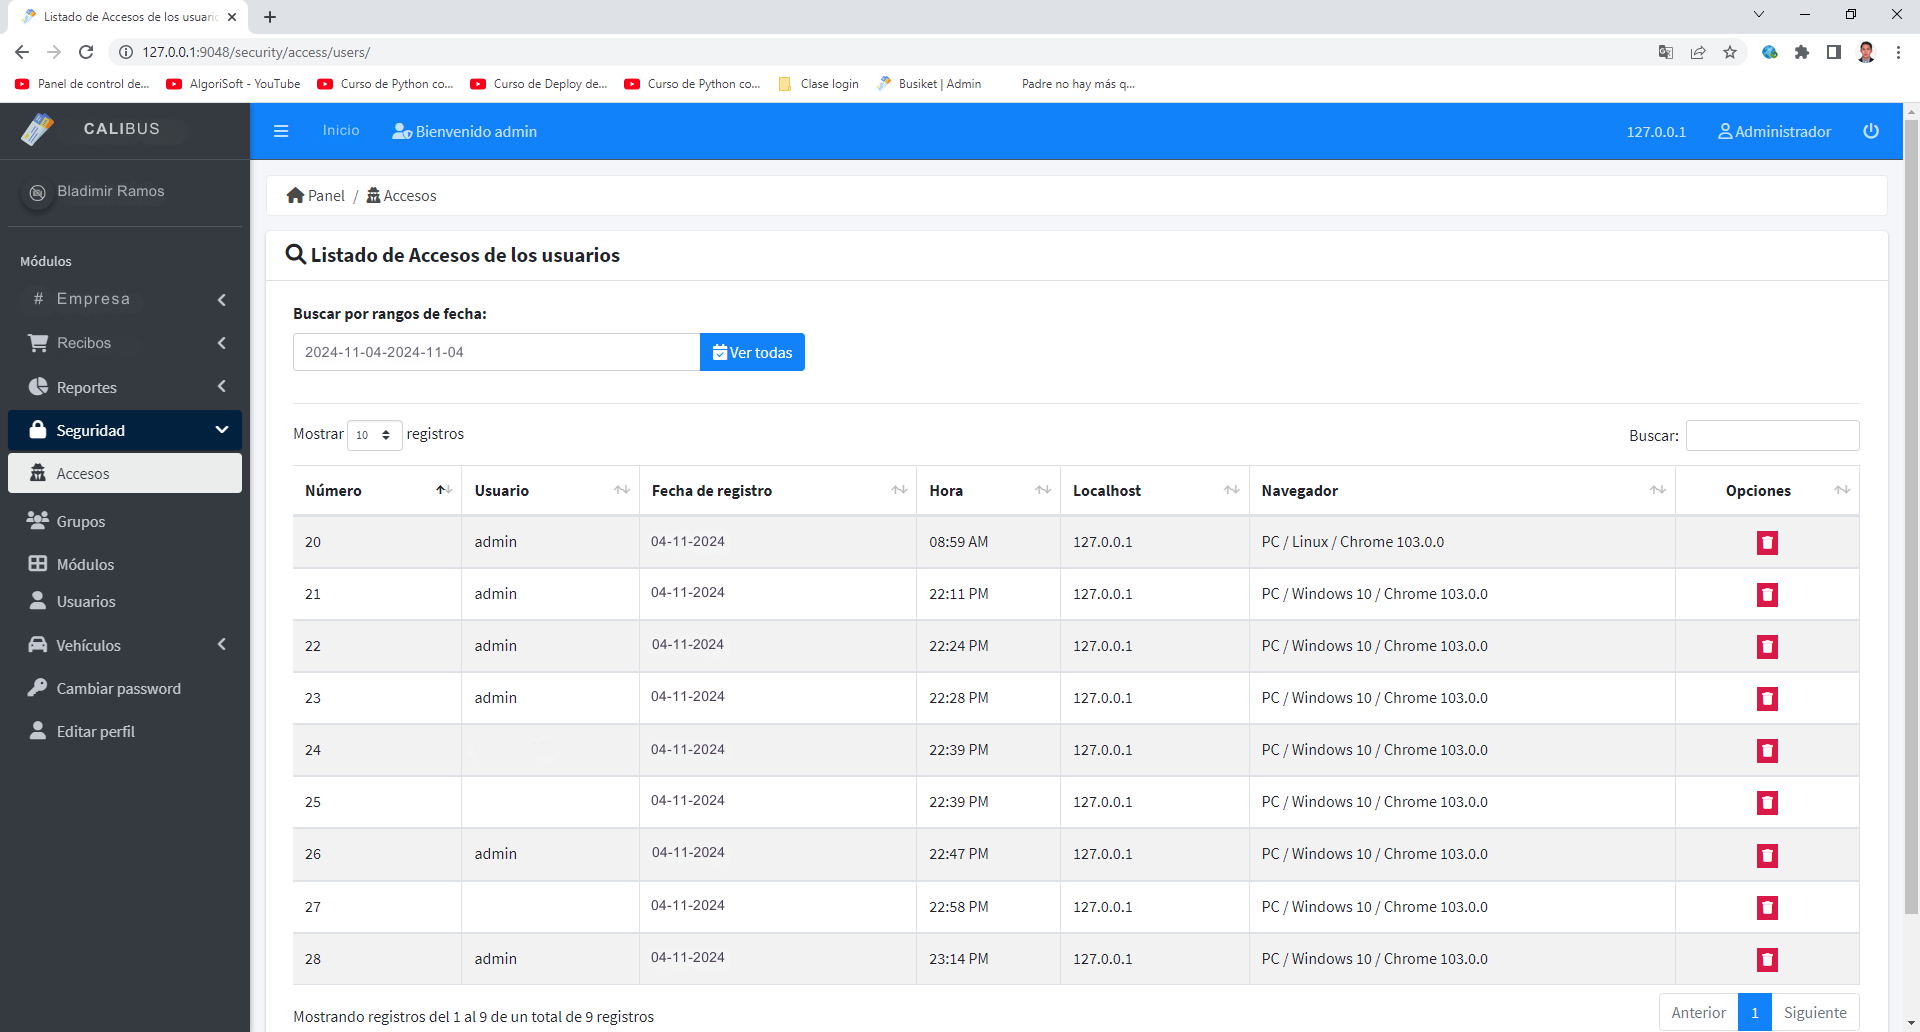
\includegraphics[width=0.83\textwidth]{imagenes/cap_3/Img_calibus/CALIBUS18.png} % Inserta una imagen
		\begin{flushleft}
			\hspace{1.20cm} \textbf{Nota.} La figura muestra la lista de accesos de los usuarios al sistema. % Nota al pie para esta figura
		\end{flushleft}
		\vspace{-16pt}
		\label{fig:cali41} % Etiqueta para referencia cruzada
	\end{figure}
	
	%\vspace{0.3cm} % Agregar 1 cm de espacio entre el párrafo y la figura
	
	Este enfoque integral de seguridad garantiza la protección adecuada del sistema de gestión de transporte de pasajeros y encomiendas, cubriendo desde la autenticación básica hasta sistemas avanzados de monitoreo y respuesta ante incidentes.
		


	
%\begin{figure}[!h] % 'H' del paquete 'float' para mantener posición	
%	\caption[Interfaz gráfica - Cambio de contraseña]

%	{\newline Interfaz gráfica - Cambio de contraseña.} % Leyenda en la parte superior
%	\centering
%	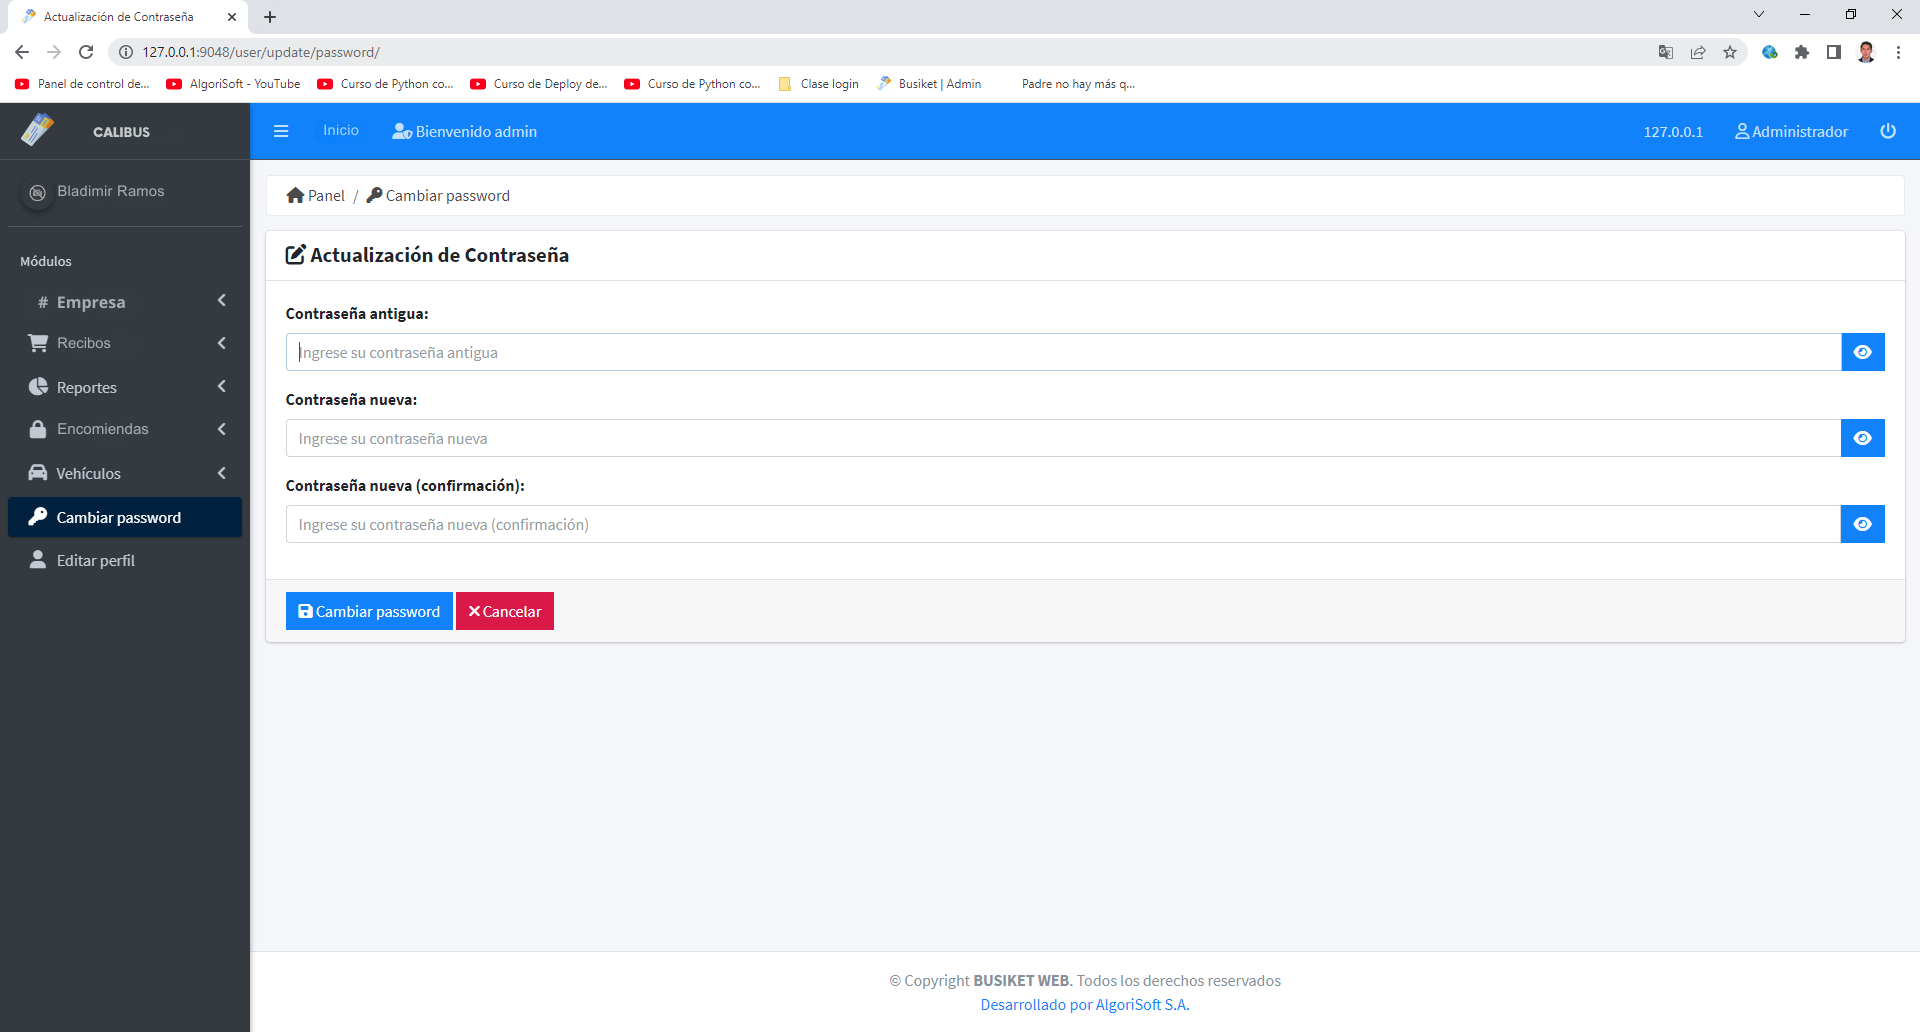
\includegraphics[width=0.85\textwidth]{imagenes/cap_3/Img_calibus/CALIBUS09.png} % Inserta una imagen
	
%	\begin{flushleft}
		%\hspace{1.20cm} \textbf{Nota.} Organigrama obtenido en entrevista con el administrador. % Nota al pie para esta figura
%	\end{flushleft}
%	\vspace{-16pt}
%	\label{fig:cali40} % Etiqueta para referencia cruzada
%\end{figure}

%\vspace{-0.6cm} % Agregar 1 cm de espacio entre el párrafo y la figura



